\chapter{System design}
\label{cha:design}
In this chapter, the design process is presented, starting from the requirements and a high-level view of the system architecture. After that, the main components of the system are described in better detail, together with the data modeling and the flow of the entire process.

The system works in the following way: it takes a list of users and their corresponding data as input, and outputs a collection of personas that represent the input users. It is designed to work with social media data: in this sense, a list of users could be the followers of a brand on a given social network, or a list of users who post about a certain topic.


\section{Requirements}
\label{sec:requirements}
The system must meet the following main requirements:
\begin{itemize}
    \item personas should be created automatically without the need of any input other than users' data;
    \item collection from multiple data sources should be supported;
    \item users of the service should be able to add new user data (or modify the already present one) for their personas, and those personas should be subsequently updated to reflect the new data;
    \item the system should be fully GDPR compliant.
\end{itemize}
As for other non-functional requirements, generated personas should accurately represent the users on which they are based. Additionally, the computation time should not be long, although data comes from an online stream of contents. Moreover, the system should be easily scalable, in case new data sources need to be supported.

\section{Main components}
\label{sec:main_components}
The system consists of five main components, which are shown in Figure~\ref{fig:logical_components}: four logical ones that sit on top of a web API. Each logical component carries out a part of the process required to go from raw data - a list of user identifiers from different social networks or other websites - to the final result - personas. The steps are the following:
\begin{enumerate}
    \item collect user data from social networks/other websites, such as demographics and activities;
    \item enrich the data with new insights derived from the results of the previous step;
    \item cluster users into similar groups;
    \item generate a persona for each cluster.
\end{enumerate}
The first two steps are coupled together, since data is sent to the enrichment module as soon as it is collected. The clustering step needs the enriched data in order to produce useful results, and the persona generator has to wait for the clusters to be created in order to carry out its job. Details on the design of each component are presented in the following sections.

\begin{figure}[t]
\centering
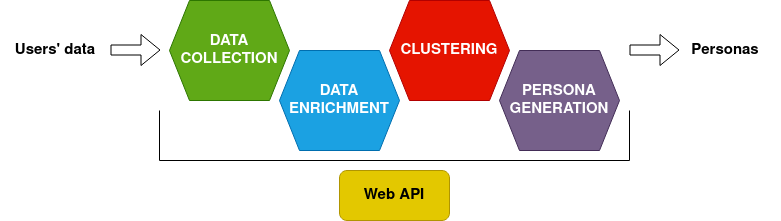
\includegraphics[width=1\textwidth]{img/Pipeline.png}
\caption{High-level view of the main components}
\label{fig:logical_components}
\end{figure}

\subsection{Data collection}
\label{subsec:data_collection}
This component has the task to fetch user data from the web. Since the system should support the creation of personas for many different contexts, the more data can be collected, the better and richer the final personas will be.

The main data source is social media data. While more traditional social networks like Twitter, Facebook or Instagram are supported for the reasons introduced in Chapter \ref{cha:art}, the system is designed to also allow the use of data from less traditional social media (e.g. Strava for sports data, Quora and Medium for user-specific blogging data). To achieve this, a list of all relevant data that can be collected needs to be defined for each data source. Relevant data can include pieces of user information such as name, location, language, number of followers, profile picture and activities (contents the user posted, complete with metadata like the number of likes, comments and shares). It should be noted that different social media usually include different data, which means there could be a lack of data if only one source is used to describe a user. In order to solve this problem, the system allows to associate multiple data sources to a single user.

Another important factor is that user data needs to be periodically collected: in fact, a huge number of activities is posted on social networks every day (around 6000 every second on Twitter\footnote{\url{https://www.dsayce.com/social-media/tweets-day/}}). For this reason, the collection component should run periodically (e.g. every 24 hours) in order to keep user data up to date and to retrieve the latest activities.

In general, this component needs as \textit{input} a series of IDs that identify the user among all the data sources associated to them. The expected \textit{output} is, for each data source, the corresponding user information and \textit{n} user activities. The number \textit{n} of activities to download could be given as a parameter, but it should not be too large in order to avoid overloading the system. For example, Twitter allows to fetch up to 200 tweets per request.

\subsection{Data enrichment}
This component has the task to derive new insights from the data that was previously collected. These insights are what users will ultimately be clustered on, which means that this phase determines how the final personas will look like. The enrichment component is split in two modules: one enriches user activities, and one enriches user profile information.

\subsubsection{Activity enrichment}
\label{subsubsec:activity_enrichment}
The goal of this module is to extract, from activity data (such as raw texts and images) and metadata, useful insights, listed in the table below. While some of them are often directly available from the collected data (such as the language or device used), the biggest challenge is to extract what the activity is about. Such information is important because it allows to gain insights on a user's behavior, such as their interests and personality. This task is further complicated when taking different forms of media (text, images) and different languages into account.

\begin{center}
\begin{tabular}{lll}
\hline
Enrichments & & \\
\hline
\textbf{String} & language & \%Language of the activity (if a text is present) \\
\textbf{Float} & sentiment & \%Value that indicates the tone of the activity \\
\textbf{Set[String]} & entities & \%Strings representing what the user talks about in the activity\\
\textbf{String} & device & \%The device on which the activity was posted \\
\hline
\end{tabular}
\end{center}

The expected \emph{input} is a user activity, as collected in the previous step. The \emph{output} is the enriched activity.

\subsubsection{User profile enrichment}
\label{subsubsec:user_profile_enrichment}
The goal of this module is to make use of whatever data is available from the collected profile information, together with the enriched activities, to extract insights that are relevant for the final personas. For the purpose of designing the system to be as general as possible, we have defined a list of attributes that are present in most persona templates available online: they are shown in the table below. It should be noted that, in many cases, some of the attributes may be impossible to extract: this depends on how much a user is active on a given social media site, and what kind of information they share.

\begin{center}
\begin{tabular}{lll}
\hline
Attributes & & \\
\hline
\textbf{String} & gender & \%Predicted gender \\
\textbf{String} & age & \%Predicted age range (e.g. 19-29) \\
\textbf{String} & type & \%Whether the user profile is of an individual or brand \\
\textbf{String} & location & \%Where the user lives \\
\textbf{String} & prefLanguage & \%The language most used by the user \\
\textbf{String} & maritalStatus & \%Whether the user is single, married, etc. \\
\textbf{Boolean} & hasChildren & \%Whether the user has children or not \\
\textbf{String} & job & \%The profession of the user \\
\textbf{String} & personality & \%Myers-Briggs personality type, encoded in 4 letters \\
\textbf{Set[String]} & interests & \%List of the top interests of the user \\
\textbf{Float} & attitude & \%Average sentiment found in the user's activities \\
\textbf{Dictionary} & activityByTime & \%How much the user is active during each day \\
\textbf{Set[String]} & activeChannels & \%Social channels where the user is most active \\
\hline
\end{tabular}
\end{center}

In order to predict attributes such as gender, age or type, machine learning classifiers can be employed. For example, gender can be predicted from a name, or from a profile picture through the use of computer vision algorithms. Life event detectors could predict a user's marital status and/or if they have children by checking if they have posted about marriage or the birth of a child. Personality can be inferred by how the user interacts with other people (as presented in section \ref{sec:enrichment}), and interests are a result of the entities and topics found in the user's activities.

The expected \emph{input} is the result of the collection of user profile information from a data source and respective enriched activities, while the \emph{output} is the enriched user profile.

\subsection{Clustering}
This component has the task to create clusters of similar users, based on the characteristics that have been extracted in the previous steps. The \emph{input} is a list of users with enriched attributes, and the expected output is composed as follows:
\begin{itemize}
    \item a mapping of each user to the corresponding cluster index;
    \item a list of \textit{representative users}, one for each cluster. A representative user is made up by the characteristics that better define a cluster. It should be noted that it can either be a real user or not, depending on the clustering algorithm. For example, in the K-Means algorithm a representative user would be a \emph{centroid}, which is defined as the average of all the users in a given cluster.
\end{itemize}
The number of clusters that are found could either be specified as a parameter by the user, or could be automatically determined by the system in order to optimize the quality of the clusters.

\subsection{Persona generation}
This component has the task to generate a persona for each cluster defined in the previous step. Since the output of the clustering component includes a list of representative users, this boils down to:
\begin{enumerate}
    \item assign realistic attributes to the representative users, in case they are not directly mapped to real users (e.g. in case a representative user is defined as the average of all users in a given cluster).
    \item give an identity to each representative user: this consists in assigning them a demographically accurate name, photo and textual description.
\end{enumerate}
The \emph{input} is a list of representative users, as output by the clustering component. The \emph{output} is a list of personas, one for each cluster/representative user. Ideally, the user should be able to specify which attributes to include in the personas, in order to tailor them to their specific needs. 

\subsection{Web API}
Users of the service interact with this layer to perform their operations. The main resources are the following:
\begin{itemize}
    \item \textbf{tokens}: they are keys used for authorizing access to protected resources;
    \item \textbf{accounts}: in order to use the service, people need to create an account. This allows them to authenticate for future API requests;
    \item \textbf{brands}: an account can create many brands. A brand is essentially a collection of users: an account can create, for example, a brand for Nutella and a brand for Coca Cola, in order to generate personas independently for the two cases;
    \item \textbf{users}: users are the objects subject to collection, enrichment and clustering. Multiple data sources can be associated to one user. Each user is associated to one and only one brand; the reason behind this is that, if users were shared between brands, an account modifying one of their users (e.g. removing a data source) would have side effects on all the other accounts whose brands include that user;
    \item \textbf{clusters} and \textbf{personas}.
\end{itemize}
In order to prevent unauthorized access to important resources like user data and brand's personas, the resources should be protected. The way in which they are protected is explained in Chapter \ref{cha:implementation}.

\section{Data models}
In this section, the data models used by the system are formalized.

\subsection{Account}
The \texttt{Account} model is composed as follows; other attributes (e.g. name) could be added if needed.
\begin{center}
\begin{tabular}{lll}
\hline
Account & & \\
\hline
\textbf{String} & accountID & \%The unique ID of the account inside the system \\
\textbf{String} & email & \%The email of the user, used for authentication \\
\textbf{String} & hashedPsw & \%Hashed password (with salt), used for authentication \\
\hline
\end{tabular}
\end{center}

\subsection{Brand}
The \texttt{Brand} model is composed as follows:
\begin{center}
\begin{tabular}{lll}
\hline
Brand & & \\
\hline
\textbf{String} & brandID & \%The unique ID of the brand inside the system \\
\textbf{String} & accountID & \%The ID of the account that created the brand \\
\textbf{String} & name & \%The name associated to this brand \\
\hline
\end{tabular}
\end{center}

\subsection{User}
The \texttt{User} model is composed as follows:
\begin{center}
\begin{tabular}{lll}
\hline
User & & \\
\hline
\textbf{String} & userID & \%The unique ID of the user inside the system \\
\textbf{String} & brandID & \%The ID of the brand the user belongs to \\
\textbf{DataSource[]} & dataSources & \%List of data sources associated to the user \\
\textbf{Attributes} & attributes & \%Enriched attributes of the user \\
\hline
\end{tabular}
\end{center}
The \texttt{Attributes} object is described in Section \ref{subsubsec:user_profile_enrichment}. User attributes are populated based on the attributes present in the user's data sources (a merging strategy needs to be defined in case of disagreements between different data sources). 

\subsection{Data Source}
As data sources can be very heterogeneous, a general \texttt{DataSource} object is defined:
\begin{center}
\begin{tabular}{lll}
\hline
DataSource & & \\
\hline
\textbf{String} & sourceID & \%The unique ID of the data source inside the system \\
\textbf{String} & sourceName & \%The name of the data source (e.g. Twitter) \\
\textbf{String} & sourceUserID & \%ID of the user in this specific data source \\
\textbf{String} & username & \%Username of the user in  this specific data source \\
\textbf{String} & from & \%ID of the oldest collected activity of the user \\
\textbf{String} & to & \%ID of the newest collected activity of the user \\
\textbf{Attributes} & attributes & \%Enriched attributes of the user in this specific data source \\
\hline
\end{tabular}
\end{center}
Then, for each particular data source that is supported, a specific object needs to be defined. For example, a \texttt{TwitterDataSource} would contain the general \texttt{DataSource} properties, plus additional ones, such as: name, location, profile image, description, website, number of followers and following.

\subsection{Activity}
The same considerations about data sources heterogeneity apply to activities. A general \texttt{Activity} model is composed as follows:
\begin{center}
\begin{tabular}{lll}
\hline
Activity & & \\
\hline
\textbf{String} & activityID & \%The unique ID of the activity inside the system \\
\textbf{String} & sourceName & \%The name of the data source where the activity is from \\
\textbf{String} & sourceUserID & \%ID of the activity in this specific data source \\
\textbf{String} & authorID & \%ID of the user (in this data source) who posted the activity \\
\textbf{Enrichments} & enrichments & \%Enriched activity properties\\
\hline
\end{tabular}
\end{center}
where the \texttt{Enrichments} model is  the one described in Section \ref{subsubsec:activity_enrichment}. A more specific \texttt{TwitterActivity} would contain additional properties, like: text, language, media, hashtags, external links, number of likes and shares.

\subsection{Cluster}
The \texttt{Cluster} model is composed as follows:
\begin{center}
\begin{tabular}{lll}
\hline
Cluster & & \\
\hline
\textbf{String} & clusterID & \%The unique ID of the cluster inside the system \\
\textbf{String} & brandID & \%The ID of the brand the cluster belongs to \\
\textbf{User[]} & users & \%List of users who belong to the cluster \\
\textbf{Attributes} & representative & \%Attributes of a user who represents the cluster \\
\hline
\end{tabular}
\end{center}

\subsection{Persona}
The \texttt{Persona} model is composed as follows:
\begin{center}
\begin{tabular}{lll}
\hline
Persona & & \\
\hline
\textbf{String} & personaID & \%The unique ID of the persona inside the system \\
\textbf{String} & clusterID & \%The ID of the cluster the persona represents \\
\textbf{String} & name & \%Name of the persona \\
\textbf{String} & photo & \%Photo of the persona \\
\textbf{String} & description & \%Brief textual description of the persona \\
\textbf{Attributes} & attributes & \%Attributes of the persona \\
\hline
\end{tabular}
\end{center}

\section{System architecture}
A diagram of the system architecture is shown in Figure \ref{fig:architecture}.

The system can be logically divided in two macro-components: the first contains the collection and enrichment components, the second contains the clustering and persona generation ones. The former is described in Section \ref{subsec:pub/sub}, due to its complexity .

The latter is less complex, since it mostly works with internal data. Each clustering (and persona generation) request is fulfilled with whatever data is available at the moment. First, clusters are generated; after that, they are passed, together with representative users, to the persona generation module. This macro-component should also be able to run periodically (e.g. every 30 minutes), in order to always keep personas updated when new user data is collected.

\begin{figure}
\centering
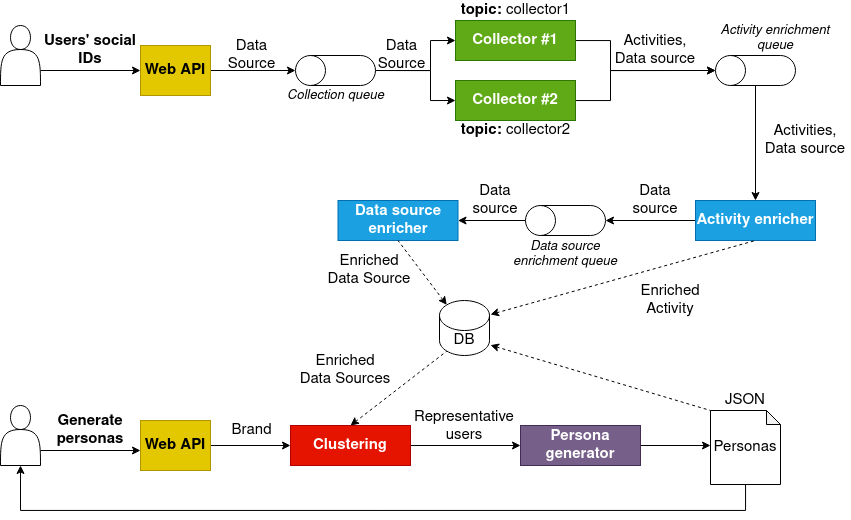
\includegraphics[width=\textwidth]{img/Architecture.png}
\caption{System architecture}
\label{fig:architecture}
\end{figure}

\subsection{Pub/Sub system for Collection and Enrichment}
\label{subsec:pub/sub}
A stream-processing design was chosen for our system. The reasons behind this choice are the following: first of all, social network data naturally falls under the category of \emph{real time data}. As mentioned in Section \ref{subsec:data_collection}, a huge number of data is posted on social networks every second, and the system would quickly get overloaded if high quantities of user data is processed in batches. Additionally, the system achieves high separation of concerns: this means that each module does not need to care about the status of other modules, and only needs to carry out its task. This also allows for the implementation of atomic, simple modules and makes the system more easily scalable and expandable, for example, in case support for a new social network needs to be added.
 
A \emph{pub/sub} (publisher/subscriber) system is one way to achieve the previously mentioned design. It consists in queues that allow communication between each module. A module can publish any kind of message on a queue with a given \emph{topic}, and all the modules that \emph{subscribed} to that topic receive the message. When one module is busy, all the incoming messages are queued and wait until they are taken by the module to be processed.

As an example, let us suppose that a user with two data sources is created through the web API: a Twitter and Facebook account. After saving the user in a database, the user ID on Twitter and Facebook are published on the \emph{collection queue}: the former is published under the topic \emph{twitter}, the latter under the topic \emph{facebook}. The Twitter and Facebook collector modules are always active, listening on the queue for their respective topics. Once the user IDs are received, the two modules independently download data, save it into the database, and publish the newly collected activities on another queue, the \emph{activity enrichment queue}. Activities are enriched, saved into the database, and once all activities of a given data source have been enriched, the data source is sent to the \emph{data source enrichment queue}. Finally, data sources are enriched and saved into the database.